%%% 修士論文(日本語)サンプル
\documentclass[dvipdfmx]{ampmt}

%%% クラスオプション:
%%% chapter: \chapterコマンドを使用可能にする(jsbook (report) を使う).
%%% その他 jsclasses に指定可能なオプションが指定できます(そのまま渡される).

%%% 題目 %%%%%%%%%%%%%%%%%%%%%%%%%%%%%%%%%%%%%%%%%%%%%%%%%%%%%%%%%%%%%%%%%%%%%%%%
\title{数理モデルの構築と効率的なアルゴリズムの開発} % 題目1行目
      {}                                             % 題目2行目
      {}                                             % 題目3行目
%%% 指導教員 %%%%%%%%%%%%%%%%%%%%%%%%%%%%%%%%%%%%%%%%%%%%%%%%%%%%%%%%%%%%%%%%%%%%
\supervisors{情報太郎}{教授}    % 指導教員1人目 {氏名}{職名}
            {工学次郎}{助教}    % 指導教員2人目 {氏名}{職名}
            {}{}                % 指導教員3人目 {氏名}{職名}
%%% 著者氏名 %%%%%%%%%%%%%%%%%%%%%%%%%%%%%%%%%%%%%%%%%%%%%%%%%%%%%%%%%%%%%%%%%%%%
\author{数理}{三郎}             % {姓}{名}
%%% 提出日 %%%%%%%%%%%%%%%%%%%%%%%%%%%%%%%%%%%%%%%%%%%%%%%%%%%%%%%%%%%%%%%%%%%%%%
\submissiondate{2021}{2}        % {年}{月}
%%% 背表紙の幅 %%%%%%%%%%%%%%%%%%%%%%%%%%%%%%%%%%%%%%%%%%%%%%%%%%%%%%%%%%%%%%%%%%
\setlength{\wdspine}{15mm}
%%% 背表紙の出力枚数 %%%%%%%%%%%%%%%%%%%%%%%%%%%%%%%%%%%%%%%%%%%%%%%%%%%%%%%%%%%%
\def\numberofspines{1}
%%% 摘要 %%%%%%%%%%%%%%%%%%%%%%%%%%%%%%%%%%%%%%%%%%%%%%%%%%%%%%%%%%%%%%%%%%%%%%%%
\abstract{
  本研究では,修士論文を執筆する学生の数理モデルを構築し,このモデルを用いて効率
  的に修士論文を作成するためのアルゴリズムを開発した.また,このアルゴリズムを用
  いて,実際に本論文を作成した.その結果,従来の自分で執筆する方法に比べて,65536
  倍効率的に修士論文を作成することが可能であることが確認された.
}
%%% パッケージの読み込みや自分用のマクロの定義 %%%%%%%%%%%%%%%%%%%%%%%%%%%%%%%%%%
\newcommand{\rme}{\mathrm{e}}
%\usepackage[top=20truemm,bottom=20truemm,left=25truemm,right=25truemm]{geometry}
\usepackage{amsmath,ascmac,url,amsfonts,bm,here,algorithmic,algorithm,amsthm,color}
\newcommand{\argmax}{\mathop{\rm argmax}\limits}
\newcommand{\argmin}{\mathop{\rm argmin}\limits} 
\newcommand{\expect}{\mathbb{E}} 
\newcommand{\trans}[1]{#1^{\top}}
\newcommand{\pdif}[2]{\frac{\partial#1}{\partial#2}}
\newcommand{\odif}[2]{\frac{\rm{d}#1}{\rm{d}#2}}
\newtheorem{th.}{定理}


%%% 出力の制御 %%%%%%%%%%%%%%%%%%%%%%%%%%%%%%%%%%%%%%%%%%%%%%%%%%%%%%%%%%%%%%%%%%

%%% 本文を出力しない場合,次の行のコメントを外して下さい.
%% \outputbodyfalse

%%% 末尾に表紙,背表紙を出力しない場合,次の行のコメントを外して下さい.
%% \outputcoverfalse

%%% 末尾に提出用摘要を出力しない場合,次の行のコメントを外して下さい.
%% \outputabstractforsubmissionfalse

%%% ampmt.cls では表紙等の作成のために geometry パッケージを使用しているため,本文
%%% のレイアウトを変えるために \usepackage[...]{geometry} とすると Option clash が
%%% 発生します.何らかの理由で本文のレイアウトを変更したい場合は \geometry{...} を
%%% 使用して下さい.
%%% また,jsclasses を使用しているため,例えば 3cm を指定したい場合は 3truecm と書
%%% く必要があります.
%% \geometry{hmargin=3truecm,vmargin=2truecm}

\begin{document}
\ifoutputbody
%%% 中表紙,摘要,目次 %%%%%%%%%%%%%%%%%%%%%%%%%%%%%%%%%%%%%%%%%%%%%%%%%%%%%%%%%%
\makeinsidecover                % 中表紙
\makeabstract                   % 摘要
\maketoc                        % 目次
\setcounter{page}{1}            % 本文のページ番号を1から始める
%%% 本文 %%%%%%%%%%%%%%%%%%%%%%%%%%%%%%%%%%%%%%%%%%%%%%%%%%%%%%%%%%%%%%%%%%%%%%%%
\section{序論}
本研究では,修士論文を執筆する学生の数理モデルを構築し,このモデルを用いて効率
的に修士論文を作成するためのアルゴリズムを開発することを目的とする.
先行研究\cite{suuri2010}を改良し,より学生の実態に合致したモデルを構築する.
また,このアルゴリズムを用いて,実際に本論文を作成する実験を行う.

\section{はじめに}
(TODO: 研究のモチベーションの整理)

\section{方策勾配を用いた強化学習}
\subsection{強化学習の基礎知識}
マルコフ決定過程$M$を$M=\{S,A,T,d_0,r,\gamma\}$として与える。ここで$S,A$はそれぞれ状態,行動集合,~$T(s^{'}|s,a)$は状態遷移確率を表す.また$d_0,r(s,a),\gamma\in[0,1]$はそれぞれ初期状態分布, 報酬, 割引率を示す.\par
さて, 強化学習の目的は
\begin{equation}
	\pi^{*}=\argmax_{\pi}J(\pi) \label{purpose_of_rl}
\end{equation}を求めることである. ここで, 
\begin{align}
	V^{\pi}(s) &= \sum_{t=0}^{\infty}\gamma^tr(s_t, a_t)|_{a_t=\pi(s_t)}, s_0 = s\\
	J(\pi) &= \expect_{s_0\sim d_0}[V^{\pi}(s_0)]
\end{align}
であり,~$J(\pi), V^{\pi}(s)$をそれぞれ評価関数, (状態)価値関数とよぶ.\par
強化学習を解析するツールとして有用な関数として$Q$関数がある.
\begin{align}
	Q^{\pi}(s,a) &= r(s, a) + \gamma\sum_{t=1}^{\infty}\gamma^tr(s_t, a_t)|_{a_t=\pi(s_t)} \nonumber\\
			    &= r(s, a) + \gamma V^{\pi}(s^{\prime}) \label{Q_func}
\end{align}
式\eqref{Q_func} より,~$Q$関数は開始時刻において自由に行動$a$を選択して, 次ステップから方策$\pi$に従った時の価値を表す. したがって,~$Q$関数は行動価値関数という別名がある.

\subsection{方策反復法}
式\eqref{purpose_of_rl}を達成するためのアルゴリズムとして方策反復法というものがある.これは以下の2つのステップを繰り返すというものである.
\begin{enumerate}
	\item 方策評価: 行動価値関数$Q^{\pi}(s,a)$を求め(または, 近似す)る.
	\item 方策改善: 求めた$Q^{\pi}(s,a)$に従って, ~$\pi(s)=\argmax_aQ^{\pi}(s,a)$と方策を更新する.
\end{enumerate}
以上の2ステップを繰り返すことで最適方策$\pi^{*}$が得られることが知られている.(方策改善定理)

\subsection{状態空間, 行動空間の特性に合わせたアルゴリズム}
\label{sec:policy_improvement}
状態空間も行動空間も離散値をとる場合,~$Q^{\pi}(s,a)$をテーブルに保存しておくことで, 前節で登場した$\pi(s)=\argmax_aQ^{\pi}(s,a)$を容易に求めることができる.\par
では, 状態空間が連続値の場合はどうか. 状態$s$が無限種類の値をとることになるため, テーブルに保存することができない. そこでMinhら\cite{DQN}は, $Q^{\pi}(s,a)$をニューラルネットワークを用いてパラメトライズして近似するアプローチをとった. ここでも, 行動空間は離散であるため$\argmax_aQ^{\pi}(s,a)$を求めることは可能である.\par
最後に, 状態空間も行動空間も連続値である場合は$\argmax_aQ^{\pi}(s,a)$を求めるのに膨大なコストがかかるという問題点がある. したがって, これまでは方策$\pi$は$Q$関数によって定めていたが, 両空間が連続値の場合にはこのアプローチはとれない. そこで, 方策関数も独立に$\pi_{\theta}$のようにパラメトライズした関数として用意し,~パラメータ$\theta$を勾配法などで更新する手法が取られることが多い.

\subsection{方策勾配による方策関数のパラメータの更新}
Silverら\cite{DPG}は, 方策が$\pi(s)$のように決定論的に定めるものとして与えた場合に, 評価関数$J(\pi_{\theta})$に対する勾配を計算する手法を発見した. この勾配は決定論的方策勾配(DPG:Deterministic Policy Gradient)とよばれ, 以下のように計算することができる.
\begin{align}
	\nabla_{\theta}J(\pi_{\theta}) &= \expect_{s\sim\rho^{\pi_{\theta}}}[
	\nabla_{\theta}\pi_{\theta}(s)\nabla_{a}Q^{\pi_{\theta}}(s, a)|_{a=\pi_{\theta}(s)}] \label{true_pg} 
\end{align}
ただし, 
\begin{equation}
	\rho^{\pi_{\theta}}(s) = \int_{S}\sum_{t=0}^{\infty}\gamma^td_0(s_0)\textrm{Pr}(s_0\to s, t,  \pi_{\theta})\textrm{d}s_0
\end{equation}
を割引分布という.\par
この方策勾配を深層強化学習の枠組みに取り入れたアルゴリズムがDDPG(Deep DPG)\cite{DDPG}である.これはActor-Critic構造を採用しており,~$Q^{\pi_{\theta}}$を近似するcriticネットワーク$Q(s,a|\omega)$と,方策$\pi$を表現するactorネットワーク$\pi(s|\theta)=\pi_{\theta}$をそれぞれ学習する手法である. 以下に,この近似勾配を用いたactorとcriticの更新アルゴリズムを記す.\par
DDPGはミニバッチ学習を用いる. 過去の経験データ$(s_t, a_t, r_t, s_{t+1})$を保存しておき, その中から$N$個のデータを取り出し(ミニバッチ, $E$と記載する),そのデータ集合に対する最適化を行う. まず, criticの更新から記す.~criticの目的は$Q^{\pi}$を近似することである.~$Q$関数は式\eqref{Q_func}のように分解することが可能で有るため,~$Q(s,a|\omega)$もこれを満たすように更新すればよい.そのためにTD(Temporal Difference)誤差
\begin{equation}
	\textrm{TD} = Q(s,a|\omega) - \{r(s,a)+\gamma Q(s,\pi(s)|\omega)\}
\end{equation}
が最小となる方向に$\omega$を更新する. 全ての$(s,a)$についてこれを一度に行うことはできないので, 作成したミニバッチ$E$に対する平均二乗誤差
\begin{equation}
	Loss = \frac{1}{N}\sum_{s\in E} \textrm{TD}^2
\end{equation}
をLoss関数として, このLoss関数を減らすようにアルゴリズムを働かせる. \par
さて, 上記のcriticの更新方法は教師あり学習そのものである. 従ってミニバッチに含まれるデータはi.i.d.であることが要求される. もしミニバッチ$E$がエージェントが経験した直近の$N$ステップのデータを用いると, これらは独立ではなくなってしまう. 従って, エージェントは環境とのインタラクションによって得られた経験データをexperience replayに保存しておき, そこから無作為に$N$このデータを選びとる手法でデータの分散を上げている.\par
次にactorの更新を記す.~actorは方策関数$\pi(s)$を表現するものであり, パラメータの更新には方策勾配を用いる.ただし,~DDPGでは式\eqref{true_pg}のように正しい$Q$関数を用いることができないので, 
\begin{equation}
	\expect_{s\sim\rho^{\pi}}[\nabla_{\theta}\pi_{\theta}(s)\nabla_{a}Q(s, a|\omega)|_{a=\pi_{\theta}(s)}] \simeq \nabla_{\theta}J(\pi_{\theta}) 
\end{equation}
のようにcriticネットワークを用いて近似した方策勾配を用いる. さらに, 期待値に関して, 
\begin{equation}
	\expect_{s\sim\rho^{\pi}}[\nabla_{\theta}\pi_{\theta}(s)\nabla_{a}Q(s, a|\omega)|_{a=\pi_{\theta}(s)}] \simeq \frac{1}{N}\sum_{s\in E}[\nabla_{\theta}\pi_{\theta}(s)\nabla_{a}Q(s, a|\omega)|_{a=\pi_{\theta}(s)}]
\end{equation}
という近似も行っている. 従って, この近似勾配$g=\frac{1}{N}\sum_{s\in E}[\nabla_{\theta}\pi_{\theta}(s)\nabla_{a}Q(s, a|\omega)|_{a=\pi_{\theta}(s)}]$はcriticの近似精度とミニバッチの分布によって大きく性能を落としてしまう可能性があり, 大きな問題点であると言える.

\section{最適セルフトリガー制御問題に対する強化学習}
\subsection{セルフトリガー制御}
図\ref{image}のような制御系を考える.
\begin{figure}[h]
	\centering
 	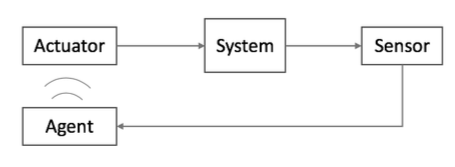
\includegraphics[width=10cm]{event.png}
 	\caption{制御系} \label{image}
\end{figure}\par
これに対するフィードバック制御を考える. 状態変数$s$を観測してアクチュエータに入力信号を送信することを「インタラクション」と呼ぶと,セルフトリガー制御では, 連続的なインタラクションは行わずに, 次のインタラクションを何秒後に行うかをエージェントが決定する. それを数式上で表すため, エージェントの制御則$\pi(s)$は2つの要素からなるベクトル値関数であるとし, 1つ目の要素はアクチュエータに送信する入力$a$,~2つ目の要素は次にインタラクションを行うまでの時間間隔$\tau~(s:秒)$を表すものとする.また, 次のインタラクションを行う時刻までは1つ前のインタラクションで送信した入力$a$を加え続けるものとする(ZOH制御).

\subsection{最適セルフトリガー制御}
最適なセルフトリガー制御則$\pi^{*}$を, 以下のように定義する. 
\begin{align}
	\pi^{*} &= \argmax_{\pi}J(\pi) \label{optimal_policy}\\
	J(\pi) &= \expect_{s_0\in d_0}[V^{\pi}(s_0)] \\
	% V^{\pi}(s_0) &= \sum_{i=0}^{\infty} \gamma^i\{-s_i^{\top}Qs_i-\pi_1(s_i)^{\top}R\pi_1(s_i)+\lambda \pi_2(s_i)\} \\
	V^{\pi}(s_0) &= \sum_{i=0}^{\infty} \gamma^i r^{\pi}_i \label{value} \\
	r^{\pi}_i &= -\int_{T_i}^{T_{i+1}}s(t)^{\top}Qs(t)\textrm{d}t +\tau_ia_i^{\top}Ra_i + \lambda \tau_i, ~T_i = \sum_{l=0}^{i} \tau_l \label{reward}
\end{align}
ここで, $i$はインタラクションの回数を示し, $a_i, \tau_i$はそれぞれ$i$回目のインタラクションでの方策$\pi$の出力であるとする. \par
さて, 一般的に強化学習では, 1ステップ1ステップの行動の良し悪しを評価して方策を更新していく. 
インタラクションとインタラクションの間の区間を「インターバル」と呼ぶと, 式(\ref{value})より, この問題は各インターバルを1ステップとした強化学習問題であると考えることができる. \par

\section{数値実験}
上記の問題は, 一般的な強化学習のフレームワークにそのまま落とし込むことができるため, 数値実験を行うことが可能である. 数値実験の結果を通して, 最適セルフトリガー制御の強化学習にどのような課題点があるのかを考察していく.\par
実験環境はOpen-AI Gymのpendulumで, 初期状態が$\theta\sim N(0, \pi), \dot{\theta}\sim U(-\pi,\pi)$となるような環境で行った. またreplay bufferの分散を上げるため,~10秒間の制御を1エピソードと定義し, エピソードを重ねることで経験データを増やしていく. また, pendulumは以下のようなダイナミクスに従っており入力アフィン系の非線型システムである.
\begin{equation}
	\odif{}{t}\begin{pmatrix}\theta \\ \dot{\theta}\end{pmatrix} = 
		\begin{pmatrix}\dot{\theta} \\ \frac{3g}{2l}\sin{\theta} + \frac{3}{ml^2}a \end{pmatrix} \label{pendulum}
\end{equation}

\subsection{方策関数の表現モデル}
セルフトリガー制御では, エージェントは各ステップにおいて入力信号$u$と, それを何秒間加えるかを決める$\tau$を決定する必要がある. 制御則を状態フィードバックとして与えるならば, 
\begin{equation}
	\pi(s) = \begin{bmatrix}u(s) & \tau(s)\end{bmatrix}^{\top}
\end{equation}
のようになる.\par
方策$\pi_{\theta}(s)$を表現するモデルとして, 図\ref{split_NN}のようなニューラルネットワークを用いる.
\begin{figure}[h]
	\centering
 	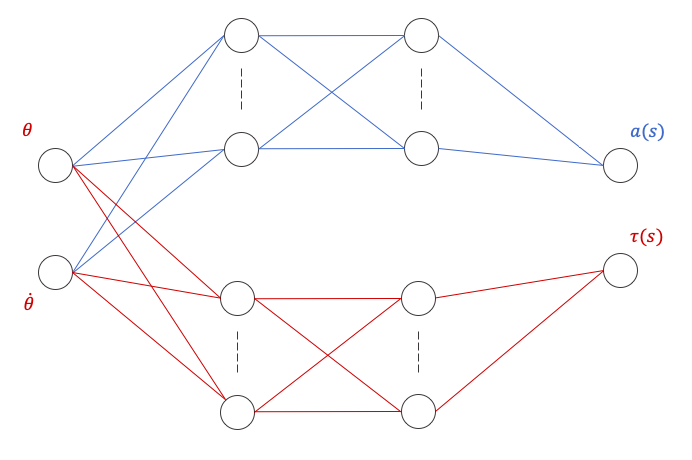
\includegraphics[width=8cm]{split_NN.png}
 	\caption{方策$\pi_{\theta}(s)$の表現モデル} \label{split_NN}
\end{figure}\\


\subsection{初期方策}
学習の初期方策として
\begin{align}
\begin{cases}
	u(s)=lqr(s)\\
	\tau(s)=0.2
\end{cases} \label{pi_init}
\end{align}
とする方策$\pi_{\rm{init}}$を用いる.ただし, $lqr(s)$はシステム\eqref{pendulum}を,離散化幅$\delta_t=0.05$として離散化したシステムを原点付近で安定化する制御則として与える.

\subsection{学習によって得られた方策}
前節まで述べてきた設定により, DDPGを用いて強化学習を行った. その結果得られた方策$\pi_{\textrm{RL}}$の制御性能を図\ref{control_path}に示す. 
\begin{figure}[h]
	\centering
 	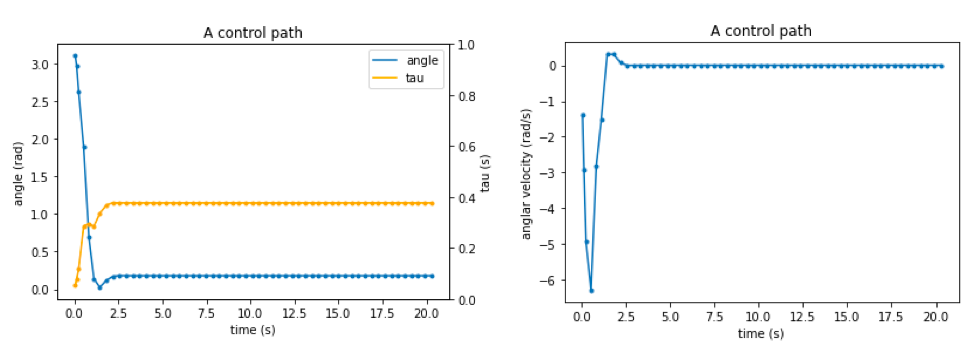
\includegraphics[width=12cm]{control_path.png}
 	\caption{学習方策$\pi_{\textrm{RL}}$による制御例} \label{control_path}
\end{figure}\\
図\ref{control_path}の左図には, 制御時間に対する角度と通信間隔$\tau$の変化をプロットしている. また, 通信が行われた時刻に点を打っている. この図から, 角度の絶対値が大きい時には細かく通信を行い, 角度が0に近い時には通信間隔を大きくするような制御を行っていることがわかる. \par
さて, この方策$\pi_{\textrm{RL}}$は, 初期方策に比べて評価関数$J(\pi)$を大きくできているのか確認する. $J(\pi) = \expect_{s_0}[V^{\pi}(s_0)]$であったので, 初期状態$s_0$を500個発生させて$V^{\pi}(s_0)$を計算した時の平均をとる作業を1000回行った. その時の結果は
\begin{equation}
	J(\pi_{\textrm{init}}) = 4.23 \pm 0.083,~J(\pi_{\textrm{RL}}) = 37.12 \pm 0.071 \label{compare_policy}
\end{equation}
となり$J(\pi_{\textrm{init}}) < J(\pi_{\textrm{RL}})$であることから, 方策改善ができていると結論づけられる. 

\section{課題点の抽出}
\subsection{方策の最適性}
前節で述べた方策$\pi_{\textrm{RL}}$は最適解なのだろうか. もし最適解であれば方策勾配が$\bm{0}$となる必要があるため, 式\eqref{true_pg}より,
\begin{equation}
	\nabla_a Q^{\pi_{\textrm{RL}}}(s,a)|_{a=\pi_{\textrm{RL}}(s)} = \bm{0}
\end{equation}
となるはずである. \par
%%% ???????
さて, 強化学習の最中は方策が各ステップで変化し続けるため, criticの近似対象となる$Q^{\pi}(s,a)$も絶えず変化していく. そのため, 正しく$Q^{\pi_{\textrm{RL}}}(s,a)$を近似できている保証はない. そこで, 方策を固定してインタラクションすることによって発生させたデータのみを用いて, ~criticを教師あり学習して$Q^{\pi_{\textrm{RL}}}(s,a)$を学習させた. この関数を$Q_{\textrm{ap}}^{\pi_{\textrm{RL}}}(s,a)$とする.\par
$\pi_{\textrm{RL}}$が最適方策であれば,~$\nabla_aQ_{\textrm{ap}}^{\pi_{\textrm{RL}}}(s,a) = \bm{0}$となるはずなので, その計算を行ってみると
\[\nabla_aQ_{\textrm{ap}}^{\pi_{\textrm{RL}}}(s,a) = \begin{bmatrix}0.03, 0.07\end{bmatrix}\]
となり, 最適解ではないことがわかった.
\par
%%%

\subsection{$Q$関数の近似精度}
$Q$関数は方策勾配

\[\nabla_{\theta}J(\pi_{\theta}) = \expect_{s\sim\rho^{\pi_{\theta}}}[
	\nabla_{\theta}\pi_{\theta}(s)\nabla_{a}Q^{\pi_{\theta}}(s, a)|_{a=\pi_{\theta}(s)}] \]

を計算するために用いられるのであった. したがって, $Q$関数の$a$に関する勾配の$a=\pi(s)$における値が,~$\rho^{\pi_{\theta}}$のサポートとなる状態$s$に対して近似できていれば良い. \par
強化学習によって得られたcriticネットワークの$Q$関数の近似が, 上記の性質を満たしているか確認する為, 図\ref{heatmap}に,~$Q(s,a|\omega)とQ_{\textrm{ap}}^{\pi}(s,a)$のそれぞれに対して$s=[0,0]$における関数値をヒートマップとして表し, $a=\pi(s)$における勾配を黄矢印にて示す.
\begin{figure}[h]
	\centering
 	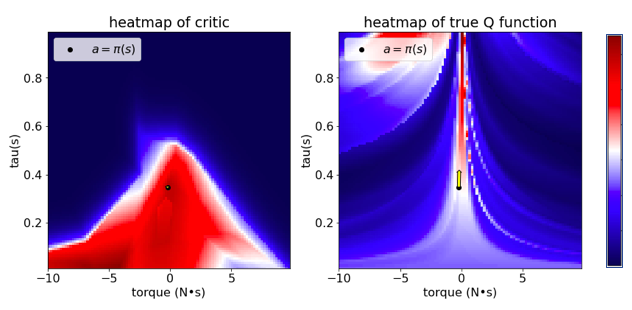
\includegraphics[width=13cm]{heatmap.png}
 	\caption{$s=[0,0]$に対する$Q$関数の近似精度} \label{heatmap}
\end{figure}\\
図\ref{heatmap}の左図は$Q(s,a|\omega)$, 右図は$Q_{\textrm{ap}}^{\pi_{\textrm{RL}}}(s,a)$を示している. 左右の黄矢印を比較すると, ~criticは$Q$関数の$a$勾配を近似できていないことが見て取れる.

\subsection{$Q$関数の近似精度が低い理由}
前節で確認した,~$Q$関数の近似精度の低さの原因はどこにあるのだろうか. まず,~criticは損失関数
\[L=\frac{1}{N}\sum_{(s,a)\in E}\{Q(s,a|\omega) - \{r(s,a)+\gamma Q(s^{\prime},\pi(s^{\prime})|\omega)\}^2\]
を小さくするように, パラメータ更新をするのであった. この最適化はデータ集合$E$に含まれる$(s,a)$にのみ働くため,その分布に存在しない領域の$(s,a)$に対する近似精度は当然低くなる.\par
では, 実際にcriticの教師あり学習に用いられたデータの分布を確認してみる. $(s,a)$は4次元のデータであるから, 可視化のために図\ref{data_distribution}では$s=[0,0]$の付近で加えられた入力$a$の分布を示している.
\begin{figure}[h]
	\centering
 	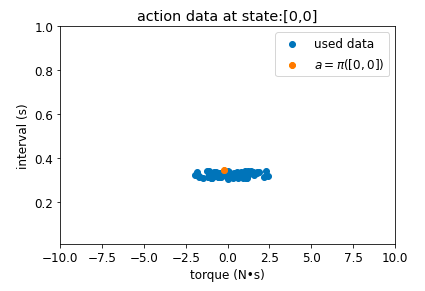
\includegraphics[width=8cm]{data_distribution.png}
 	\caption{criticの学習に用いられた$s=[0,0]$に対する行動$a$の分布} \label{data_distribution}
\end{figure}\\\\
図\ref{data_distribution}から, 非常に狭小な領域のデータを用いて関数近似がなされていたことがわかる. これは, データ収集の際に, 状態$s=[0, 0]$で加えた入力が偏っていたことが原因である. 方策勾配の計算には
\[\nabla_{a} Q(s,a|\omega)|_{a=\pi_{\theta}(s)}\]
の近似精度が肝要なので, 図\ref{data_distribution}において橙色の点で表した$a=\pi_{\theta}(s)$周りのデータが不足していることが問題となる.



\section{探索手法の工夫}
前節で過去の経験データのにおける$a=\pi_{\theta}(s)$周りのデータが欠損に不足があることを確認した. 経験データの分散を上げる為に, 各状態で多様な入力を試してみることを探索といい, まずはその探索について考えていく.
\subsection{探索}
強化学習における探索手法として「$\varepsilon$-greedyアルゴリズム」などがよく知られているが,
本稿で考えているような連続行動空間の強化学習では
\begin{equation}
	a = \pi_{\theta}(s) + e
\end{equation}
のように,方策関数の出力にノイズ$e$を付加して決定された行動でデータ収集を行うのが一般的である. (ノイズを付加した方策を, 学習中の方策と区別するために行動方策とよぶ.)直感的に, このノイズが大きければ大きいほど探索の幅が広がるため, $a=\pi_{\theta}(s)$周りのデータの分布が広がることで, ~$Q$関数の$a$に関する勾配の近似精度が向上することが予想できる. では強化学習アルゴリズム全体に対して, 探索ノイズを大きくすることはどのような影響を与えるのかについて次節で考察していく.

\subsection{探索ノイズの大きさ}
探索ノイズを大きくすれば, ~$Q$関数の$a$に関する勾配の近似精度を向上させられることを予想した. では, 探索ノイズを大きくすればそれで良いのか. 答えはNOである. 大きな探索ノイズを加えれば, 経験データ$E$の分布は割引分布$\rho^{\pi}(s)$から大きく乖離することになる. これはどのような問題を引き起こすのか.\par
actorの更新に用いる方策勾配の計算には,~$Q^{\pi}$のcriticによる近似の他にも, 以下のように状態$s$に対する期待値のサンプル平均による近似も用いられる.
\[
\expect_{s\sim\rho^{\pi_{\theta}}}[\nabla_{\theta}\pi_{\theta}(s)\nabla_{a}Q(s, a|\omega)|_{a=\pi_{\theta}(s)}] \simeq \frac{1}{N}\sum_{s\in E}[\nabla_{\theta}\pi_{\theta}(s)\nabla_{a}Q(s, a|\omega)|_{a=\pi_{\theta}(s)}]
\]
よって, 経験データ$E$の分布は割引分布$\rho^{\pi_{\theta}}(s)$に等しいことが望ましい. 従って, 入力に大きなノイズを加えることは,方策勾配の近似に対しては望ましくない操作であると言える.

\subsection{理想ケースとそれを達成する工夫}
\label{sec:proposed_method}
これまで考察してきたことをまとめると, DDPGにおいて最も理想的な経験データ集合$E$の分布は
\begin{enumerate} 
	\item 状態$s$の分布は, 割引分布$\rho^{\pi}(s)$に近い
	\item 各状態$s$に対して, ~行動$a$の分散が大きい
\end{enumerate}
を満たすものであると考えられる.% 新しい状態を見なくてもいいのか? -> もしsから離れるような行動が最適なんだったら, そこを通るような方策になってから経験すべき
そこで「入力$a$を変えても,次ステップの状態$s^{\prime}$が大きく変わらない場合」は大きなノイズを加え, 「入力$a$を変えると,次ステップの状態$s^{\prime}$が大きく変わってしまう場合」はノイズは小さくすれば, 上記の要求を満たす経験データ集合を構築できるのではないか.\par
例えば, 探索ノイズを正規乱数$\mathcal{N}(0,1)$のスカラー倍として与える場合に, そのスカラー$k$(以下ノイズスケールと記載)を適応的に変化させることを考える. 次ステップの状態$s^{\prime}$は, 現在の状態$s$と入力信号$u$および通信間隔$\tau$の関数として与えられるので, 
\[\pdif{s^{\prime}}{u}, \pdif{s^{\prime}}{\tau}\]
の大きさによって, ~$u,\tau$それぞれに加えるノイズスケール$k_u, k_{\tau}$を適応的に与えれば良い. \par
% スパイスとしてセルフトリガーだからこそのことが言いたい

\subsection{提案手法による実験結果と考察}
\ref{sec:proposed_method}節で提案した探索手法を用いて強化学習を行い, それにより得られた方策を$\pi_{\textrm{prop}}(s)$を表記すると, その評価関数$J(\pi_{\textrm{prop}})$の値は, 
\begin{equation}
	J(\pi_{\textrm{prop}}) = 68.10 \pm 0.018
\end{equation}
となり, 式\eqref{compare_policy}における$J(\pi_{\textrm{RL}})$からの改善が見られた.


\subsection{提案手法の妥当性の検討}
\ref{sec:proposed_method}節で提案した探索手法は, 次ステップの状態が方策$\pi_{\theta}(s)$で制御を行った場合から, 大きく変化することを避けることを目的としていた. これは新たな状態を経験しないことになるので, 果たして探索と言えるのであろうか.\par
\ref{sec:policy_improvement}節で述べたように, 連続行動空間では
\begin{equation}
	\pi(s) \gets \textrm{argmax}_{a} Q^{\pi}(s,a)
\end{equation}
として方策改善をすることは難しい. そこで方策勾配法を用いて方策改善を行う手法をとっていた. したがって, 連続行動空間の強化学習においては, エージェントは「いち早く、最適な状態行動組を経験する」ことよりも, 「方策勾配を正しく計算する」ことを優先すべきである. よって, 提案手法には妥当性があると考えられる.



\section{まとめ}
本稿では, 最適セルフトリガー制御を定式化し, その強化学習による解法を試した. それにより得られた方策や, 方策勾配の近似に用いられた関数などを解析することにより, 課題点の抽出とその原因の特定を行った. さらに, 抽出した課題点に対する解決策の提案も行った. \par
しかしながら, 本稿で提案した手法は強化学習一般の課題点を解決するためのものであり, またその提案手法も, 本稿で定式化した最適セルフトリガー制御にユニークな特徴を活かしていない. 今後は有効な特徴がないか調査していきたいと考える. \par
また方向では, DDPGにおける「探索」のモチベーションを,~$\nabla_{a} Q^{\pi}(s,a)|_{a=\pi(s)}$の近似のみにあると仮定して議論を行った. この妥当性についても検討していきたい.

%%% 謝辞 %%%%%%%%%%%%%%%%%%%%%%%%%%%%%%%%%%%%%%%%%%%%%%%%%%%%%%%%%%%%%%%%%%%%%%%%
\acknowledgment
本研究に取り組むにあたって助言をいただいた情報太郎教授と工学次郎助教に深く感謝
する.

%%% 参考文献 %%%%%%%%%%%%%%%%%%%%%%%%%%%%%%%%%%%%%%%%%%%%%%%%%%%%%%%%%%%%%%%%%%%%
\addcontentsline{toc}{section}{\refname} % 目次に参考文献を追加する.
                                         % chapter使用時は削除すること.
\begin{thebibliography}{10}
\bibitem{Q}
C. J. Watkins, and P. Dayan. Q-learning. \textit{Machine Learning}, vol. 8, no. 3-4, pp. 279-292, 1992.
\bibitem{DQN}
V. Minh, K. Kavukcouglu, D. Silver. et al.. “Human-level control through deep reinforcement learning." \textit{Nature 518}, pp.529-533, 2015.
\bibitem{DPG}
D. Silver, G. Lever, N. Heess, T. Degris, D. Wierstra, et al.. “Deterministic Policy Gradient Algorithms." \textit{ICML Beijing, China.}, 2014, Beijing.
\bibitem{DDPG}
T. P. Lillicrap, J. J. Hunt, A. Pritzel, N.Heess, T. Erez, Y. Tassa, D. Silver, and D. Wierstra. Continuous control with deep reinforcement learning. \textit{International Conference on Learning Representations}, 2015.
\bibitem{off-PAC}
T. Degris, M. White and R. Sutton. “Off-Policy Actor-Critic." \textit{ICML Edinburgh, United Kingdom}, 2012.
\bibitem{approximation}
R. S. Sutton, D. McAllester, S. Singh, and Y. Mansour. "Policy gradient methods for reinforcement learning with function approximation." \textit{In Advances in Neural Information Processing Systems}, 2000.
\bibitem{Adam}
D. P. Kingma and J. Ba. “Adam: A Method for Stochastic Optimization." \textit{arXiv preprint arXiv: 1412.6980}, 2014.
 
\end{thebibliography}
%%% BibTeX 等を用いる場合は,上の thebibliography 環境を消してここに該当コードを
%%% 挿入すること.
%% \bibliographystyle{...}
%% \bibliography{...}

%%% 付録 %%%%%%%%%%%%%%%%%%%%%%%%%%%%%%%%%%%%%%%%%%%%%%%%%%%%%%%%%%%%%%%%%%%%%%%%
%%% 付録は不要ならば削除してよい.
\appendix
\section{aho}









%%% 本文ここまで %%%%%%%%%%%%%%%%%%%%%%%%%%%%%%%%%%%%%%%%%%%%%%%%%%%%%%%%%%%%%%%%
\fi
\ifoutputcover
\cleardoublepage
%%% 表紙,背表紙,提出用摘要 %%%%%%%%%%%%%%%%%%%%%%%%%%%%%%%%%%%%%%%%%%%%%%%%%%%%
\makecover                      % 表紙
\makespine[\numberofspines]     % 背表紙
\fi
\ifoutputabstractforsubmission
\makeabstractforsubmission      % 提出用摘要
\fi
\end{document}
